%%%%%%%%%%%%%%%%%%%%%%%% CAB432 Group Report %%%%%%%%%%%%%%%%%%%%%%%

%BEGIN_FOLD
% Disclaimer: You HAVE to use this. This is a not simple starting point, all libraries and titles were recreated for fit group Assignment, same way it was in EGB342. If something does not work... Well, you all know who to blame.

% This sets the style of the document, you can use different built in styles, create your own .cls files or download ones from the Internet. This one is fairly standard to use
\documentclass[12pt]{article}
\usepackage[natbibapa]{apacite}


%%%%%%%%%%%%%%%%%%%%%%%%%%%%% Packages %%%%%%%%%%%%%%%%%%%%%%%%%%%%%%

% This package is handy for captioning figures, you can set caption style here as well
\usepackage[font={small,it}]{caption}
\usepackage[a4paper, portrait, margin=0.8in,top=2cm,bottom=2cm,]{geometry}
\usepackage{bigstrut}

% This is important for position images as latex will put your image where it best fits unless you tell it otherwise
\usepackage{float}
\usepackage{wrapfig}

% If you want images this is necessary
\usepackage{graphicx}
\usepackage{subcaption}
\graphicspath{{./images}}
\usepackage{hyperref}
\usepackage{color}
\usepackage{xcolor}
\hypersetup{colorlinks=true}
\hypersetup{linkcolor=blue}
\newcommand\PlaceText[3]{%
\begin{tikzpicture}[remember picture,overlay]
\node[outer sep=0pt,inner sep=0pt,anchor=south west] 
  at ([xshift=#1,yshift=-#2]current page.north west) {#3};
\end{tikzpicture}%
}
% You can use this to set your margin size
%\usepackage[margin=25mm]{geometry}

% Allows you to do things such as headers and footers
\usepackage{fancyhdr}

% This needs to be in here if you want to set up your document with more than one column in sections 
\usepackage{multicol}

% Here are a few packages that help with formatting equations, you may not need to use this but I find align* from amsmath particularly useful
\usepackage{amsmath,amssymb,amsthm,textcomp,amsfonts,amsthm,mathrsfs}
\usepackage{xparse}% http://ctan.org/pkg/xparse
\NewDocumentCommand{\ceil}{s O{} m}{%
  \IfBooleanTF{#1} % starred
    {\left\lceil#3\right\rceil} % \ceil*[..]{..}
    {#2\lceil#3#2\rceil} % \ceil[..]{..}
}

% Enhances Latex`s cross referencing
\usepackage{cleveref}
\usepackage{hyperref}
\hypersetup{colorlinks=true}
\hypersetup{linkcolor=blue}
\usepackage{xcolor}
\usepackage{physics}
\usepackage{gensymb}
\usepackage{mathrsfs}

% Also not necessary but I find it handy when formatting arrays and matrices
\usepackage{array}
\usepackage{xfrac}
\usepackage{enumitem}

%% These packages you`ll need to download a .sty file before you can use

% This allows really nice formatting for MATLAB code.
\usepackage[numbered,framed]{mcode}
\usepackage{mathrsfs}
\usepackage{hyperref}
\hypersetup{colorlinks=true}
\hypersetup{linkcolor=blue}
\usepackage{xcolor}
\usepackage{physics}
\usepackage{gensymb}

%% Feel free to add any more packages you want!!!
\usepackage{indentfirst}
\usepackage{parskip} 
\setlength\parindent{0pt}
%\setlength{\parskip}{1cm plus4mm minus3mm}
\usepackage{csquotes}
\usepackage{mathtools}
\newcommand{\Lim}[1]{\raisebox{0.5ex}{\scalebox{0.8}{$\displaystyle \lim_{#1}\;$}}}
\usepackage{wrapfig}

%%%%%%%%%%%%%%%%%%%%%%%%% Setup the document %%%%%%%%%%%%%%%%%%%%%%%%

\lstset{basicstyle=\scriptsize\ttfamily,breaklines=true}
\renewcommand{\thesubsection}{\thesection.\arabic{subsection}.}

\renewcommand{\thesubsubsection}{\indent \roman{subsubsection}}

\numberwithin{equation}{section} % Number equations within sections (i.e. 1.1, 1.2, 2.1, 2.2 instead of 1, 2, 3, 4)
\numberwithin{figure}{section} % Number figures within sections (i.e. 1.1, 1.2, 2.1, 2.2 instead of 1, 2, 3, 4)
\numberwithin{table}{section} % Number tables within sections (i.e. 1.1, 1.2, 2.1, 2.2 instead of 1, 2, 3, 4)

\newcommand{\horrule}[1]{\rule{\linewidth}{#1}} % Create horizontal rule command with 1 argument of height

\title{	
	\normalfont \normalsize 
	\textsc{Queensland University of Technology} \\ [25pt] 
	\horrule{0.5pt} \\[0.4cm] % Thin top horizontal rule
	\huge CAB432 - Assignment 1 – Mashup Project \\ Proposal \\ % The assignment title
	\author{ Marat (Matt) Sadykov \small n9312706 \\ \\ Tutor: Jacob Marks \small \underline{marksj@qut.edu.au}}
	\date{\normalsize\today} % Today`s date or a custom date
	\horrule{2pt} \\[0.5cm] % Thick bottom horizontal rule
}
%\title{\textbf{Assignment 1}\\ \large  EGB342 \\ Group 10}
%\author{Matt Sadov \small n9312706 \\ Stephen Hannam \small n2731061\\ Thomas Nugent \small n9219986}
%\date{May 2017}


% Headers and footers
\pagestyle{fancy}
\fancyhf{}
\rhead{Mashup Proposal}
\lhead{CAB432 Cloud Computing}
\cfoot{Marat (Matt) Sadykov}
\cfoot{Page \thepage}
\cfoot{n9312706}

%END_FOLD
%%%%%%%%%%%%%%%%%%%%% Begin the Actual Document %%%%%%%%%%%%%%%%%%%%%
\begin{document}
\maketitle
\newpage
%\tableofcontents
\newpage
%===================================================%
%													%
%============ Section 1 Introduction ===============%
%												    %
%===================================================%
\section{Introduction}	
%	\begin{enumerate}
%		\item Overall mashup purpose and description (1-2 Paragraphs)
%		\item List of service and data APIs to be utilised. Short description of API (1 paragraph)
%	\end{enumerate} 

	The aim of this project to provide users with some comfortable environment to plan their journeys. This planner will use one of the following API\footnote{Names contain hyperlinks to resource. Feel free to click}: 
	
	\begin{itemize}
		\item \href{https://developers.google.com/maps/documentation/}{Google Maps}
		\item \href{https://hackathon.expedia.com/docs/public/api/Flights Overview/}{Expedian} with \href{https://partners.skyscanner.net/affiliates/travel-apis/}{Skyscanner} combined for one purpose.
		\item \href{https://developers.webcams.travel/\#webcams/list}{Webcam}
	\end{itemize}	
	A user will be able to choose a destination, view closes and cheapest flight information and makes a decision based on a picture from realtime webcameras (Maybe it is not as pretty, but it will give right feeling regarding destination). First and the important part is an interactive map, provided by Maps services. It will allow a user to change view between satellite and geographic, zoom in to view details and help to extract geographic locations. Next is the webcam, which produces some images or short video streams on some of the sights of the area. And the Main part is quick information on the closest flight regarding price, time and journey. The first experiment version is presented in Figure~\ref{fig:map}.	

	\subsection{World Map}
		The foundation for weekend planer environment is continental Map. Gladly, there is a high chance of finding a right Map provider. Two global websites, whose work offers an API for use cases are Google Maps and Yandex. If first is the global giant, who existed in the worldwide market for a while, second has the most popularity in Russian. Both of them will serve the primary purpose very well: establish a right environment for integrating other API. Besides, both services provide an excellent API to extend the scope of the current project. \\
		
		As a result, the Google Map API was chosen with a way presented in Figure~\ref{fig:gmaps}. To describe location, a centre point of the map must be chosen with longitude and latitude. In addition, API provides a good drawing environment, which allows places some images on top of the map, draw markers or lines from one location, to another. As a scope of this unit, only Aultralia will be chosen as working environment.
		
		\begin{figure}[H]
			\centering        
			\includegraphics[width=0.7\textwidth]{images/google-map}
			\caption{Google Maps API at 54 54 longitude and latitude.}
			\label{fig:gmaps}
		\end{figure}	
	\subsection{Flight Management}
			
		
		To gather information about the possible flight tickets, there is a possibility of particular problems. Since the beginning of the project, the request for API keys may take longer than expected. Such services like Expedia provides some flight information, which may be used to gather closest flight information about time, prices, airports. Obtaining this information may become a trickier process. For example, if there will be no alternatives discovered, the best solution in this situation will be parsing web page with flight information. However, this approach goes beyond the scope of the assignment, it may prove itself as a good, but not easy, alternative.\\
%		\subsubsection{Expedia}
%			Expedia, yandex - waiting.
	\subsection{Location Explorer}
		$  $ \\
		
		To gather information unusually and present in on top of maps webcam service will be used. Generally, it contains Library of open web cameras located around the world. Instead of gathering all possible sources, webcam includes all of them in one place. It will allow extracting at least images, which were made very recent to a user request. An example of how data can be collected is displayed in Figure~\ref{fig:webcam}.
%===================================================%
%													%
%============ Section 2 Use Cases ==================%
%												    %
%===================================================%
\section{Use Cases}
	\subsection{Trip Planner}
	The main expected advantage of this service is to \textbf{plan trips to several places} on one Map, instead of planning on the official website, comparing each ticket one by one. This comparison gives user possibility select option which is not only cheaper but also is flexible regarding destinations.
	
	\subsection{Exploring area with cameras}
	Web cameras spread around cities all other the place. Some of them may contain boring traffic exploration, another some beautiful views. Comparing to high-quality images on other services, webcam takes real-time shoots. The original intention is to allow the user to plan short weekend trips. \textbf{There is no better way to make desition rather take a small pick into a city of destination.}
	\begin{figure}[H]
		\centering        
		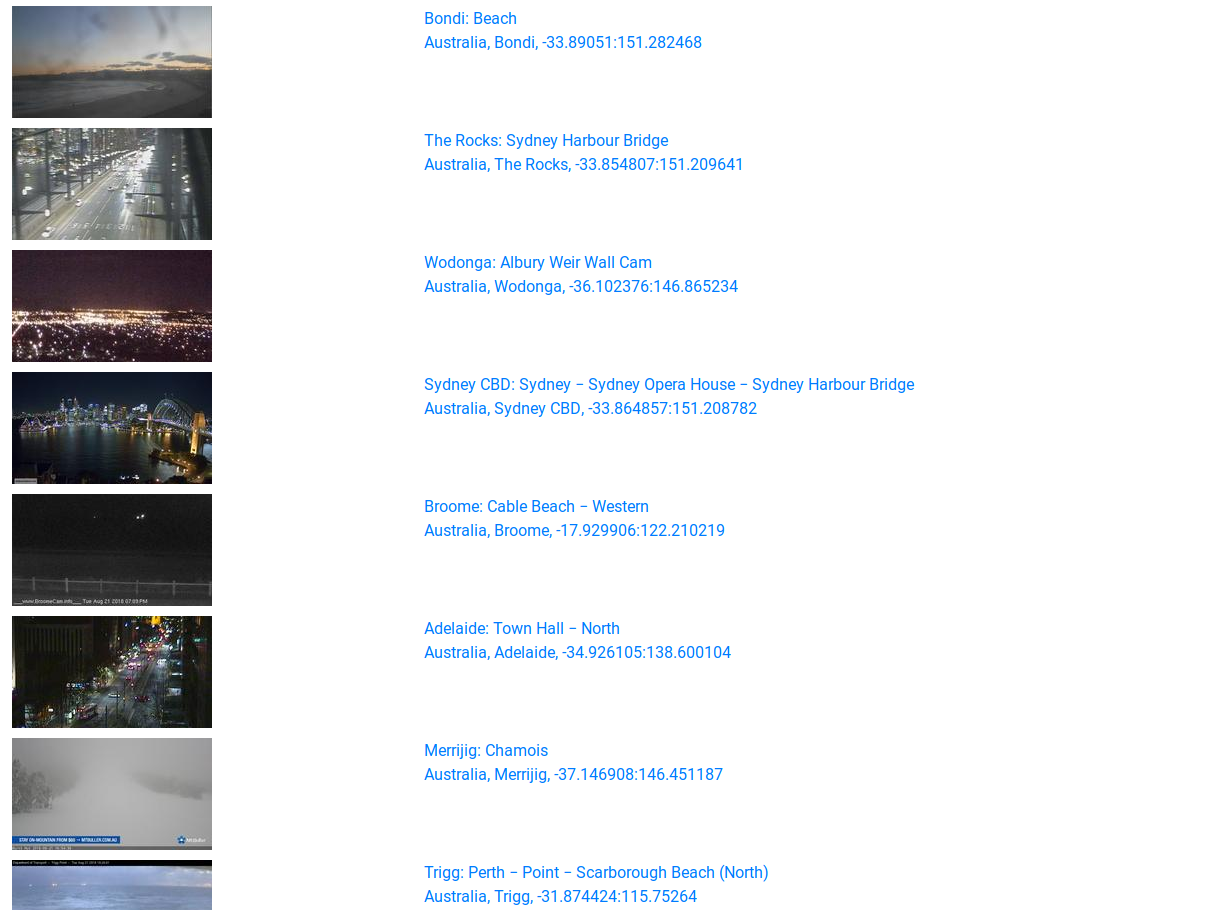
\includegraphics[width=0.7\textwidth]{images/webcam}
		\caption{First test print with API use.}
		\label{fig:webcam}
	\end{figure}
	\subsection{Weekend planner}
	In addition to flight management and camera exploration, some of \textbf{the Maps services} can be used to make decisions on sight. For example, explore the streets a destination in a particular city, without moving to another Map view. \\
	In addition to this stage of the project, final goal after implementing the server side of the project is to allow the possibility of integration this web application into Linux GNOME Desktop environment. With this opportunity, the user will be free from the browser and will be able to make a decision during weekday workflow.
	
	\begin{figure}[H]
		\centering        
		\includegraphics[width=0.7\textwidth]{images/map2}
		\caption{Part of the map with expected functionality.}
		\label{fig:map2}
	\end{figure}
		
%===================================================%
%													%
%============ Technical Breakdown===================%
%												    %
%===================================================%
\newpage
\section{Technical Breakdown}	
%	\begin{enumerate}
%		\item A clear division between Server, Client and Cloud.
%		\item  a mock-up of your application page		
%	\end{enumerate} 
	The image below~\ref{fig:break} represents the first structure breakdown of the current project. Arrow indicates application communication on client site, then dot arrows indicate web request and response. The blue connection between API and cloud services are constant communication to provide service.
	\begin{figure}[H]
		\centering		
		\includegraphics[width=\textwidth]{images/Breakdown}
		\caption{First structure Breakdown.}
		\label{fig:break}
	\end{figure}	
\newpage
\section{Client}
	Using only GET. Based only everything with Map. Passing all videos, and mnarking places. Then asking for flight, using clik. After requesting specific city, GET post send to server and server makes response to Flight.		
\section{Server}

\section{*Response Filtering}
	Everything comes depending response, and printed as per requested, based on result of send.
\section{Docker}
\section{Design}
	Design based on one of a examples, drawen by ourself, which prints results on the screen.

\section{Difficulties}
	
	\subsection{More API than necessary}
	\subsection{Asynchronic request}
\section{Future work}
	\subsection{Gnome Integration}
	\subsection{Several Extra APIs}

\section{Appendix}	
	\begin{figure}[H]
		\centering		
		\includegraphics[width=0.8\textwidth]{images/map}
		\caption{First test implementation.}
		\label{fig:map}
	\end{figure}
%	\begin{center}
%		\footnotesize\textit{i.e. a QPSK modualtion scheme}\normalfont
%	\end{center}
%
%	\begin{center}
%		\begin{tabular}{c}
%			\begin{lstlisting}[linewidth = 15cm, name = Thomas Nugent]
%				function [t, QPSK_msg, msgi, msgq, f] = QPSK_transmit(msg, start_time,...
%				Rs, Ns, A, fc)
%				\end{lstlisting}
%		\end{tabular}
%	\end{center}
%%===================================================%
%%													%
%%================= Difficulties ====================%
%%												    %
%%===================================================%
%\section{Difficulties}
%	\cite[p.~278]{GOD} \\ 
%	\cite{michelson}
%	
%	\begin{align}
%		S_{m}(t) = A_{mc}g(t)cos(2\pi f_{c}t) - A_{ms}g(t)sin(2\pi f_{c}t)
%	\end{align}
%	
%	\cite{fundcomm} This causes 
%
%	
%	\hyperref[pros_cons]{subsection further}.
%	
%	\begin{figure}[H]
%		\begin{subfigure}[b]{0.52\textwidth}
%			\centering
%			\includegraphics[width=\linewidth]{images/marie-b}
%			\caption*{8-QAM -5dB to -2dB.}
%			\label{fig:Xana}
%		\end{subfigure}
%		\begin{subfigure}[b]{0.52\textwidth}
%			\centering
%			\includegraphics[width=\linewidth]{images/Shelob}
%			\caption*{8-QAM -5dB to -2dB.}
%			\label{fig:Shelob}
%		\end{subfigure}
%		\caption{8-QAM -5dB to 16dB.}
%		\label{fig:My laptop}
%	\end{figure}
%	
%	\begin{equation}
%		Pb = \frac{4}{log_{2}M}Q\left\lbrace \sqrt{ \left( \dfrac{3(log_{2}M)}{M-1}\frac{Eb}{No}\right)}\right\rbrace
%	\end{equation}
%
%	\subsection{Subsection with label} \label{pros_cons}
%		To justify the difference with higher order schematics, it will be better to actually 	
%	
%		\begin{figure} [H]
%			\centering
%			\begin{minipage}[b]{0.45\textwidth}
%				\centering
%				\includegraphics[width=\linewidth]{images/image1}
%				\caption*{8-QAM 12dB to 16dB.}
%				\label{fig:16-QAM}	
%			\end{minipage}
%			\hfill
%			\begin{minipage}[b]{0.45\textwidth}
%				\centering
%				\includegraphics[width=\linewidth]{images/marie-b}
%				\caption*{8-QAM -4dB to 2dB.}
%				\label{fig:32-QAM}	
%			\end{minipage}
%			\begin{minipage}[b]{0.45\textwidth}
%				\centering
%				\includegraphics[width=\linewidth]{images/Shelob}
%				\caption*{8-QAM 12dB to 16dB.}
%				\label{fig:64-QAM}	
%			\end{minipage}
%			\hfill
%			\begin{minipage}[b]{0.45\textwidth}
%				\centering
%				\includegraphics[width=\linewidth]{images/UQ}
%				\caption*{8-QAM -4dB to 2dB.}
%				\label{fig:128-QAM}	
%			\end{minipage}
%			\caption{8-QAM -4dB to 2dB Main label.}
%			\label{fig:QAM-schemes}
%		\end{figure}
%%===================================================%
%%													%
%%================= Extensions ======================%
%%												    %
%%===================================================%
%\newpage
%\section{Extensions}
%
%%===================================================%
%%													%
%%=================== Testing =======================%
%%												    %
%%===================================================%
%\newpage
%\section{Testing}
%
%%===================================================%
%%													%
%%===================REFLECTIOM======================%
%%												    %
%%===================================================%
%\newpage
%\section{Reflection}
%Reflection
%
%%===================================================%
%%													%
%%===================Apeendix A======================%
%%												    %
%%===================================================%
%\newpage
%\section{Appendix A}
%Reflection
%
%%===================================================%
%%													%
%%============Bibliography and refferencing==========%
%%												    %
%%===================================================%
%\begin{flushleft}
%	\bibliographystyle{apacite}
%	\bibliography{referencing/referenceList}
%\end{flushleft}

\end{document}
